
\documentclass[journal,comsoc]{IEEEtran}
\usepackage[T1]{fontenc}
\usepackage{url}
\usepackage{graphicx}
\usepackage{float}
\ifCLASSINFOpdf
\else
\fi
\usepackage{amsmath}
\interdisplaylinepenalty=2500
\usepackage[cmintegrals]{newtxmath}
\begin{document}
\title{Ransomware: Is human error the primary reason for the surge in this increasingly popular malware?}
\author{Craig Heptinstall Crh13- 110005643\\Institute of Computer Science - Aberystywth University}
\maketitle

\begin{abstract}
As computers and other machines become more and more an integral part of a person's life, the risk of a computer infection increases. The amount of platforms available to the common user today allows malicious attackers a variety of ways to access user's personal data (from contact details to banking details.) A class of malware (malicious software) that has been reported more than others in recent years known as Ransomware has been taking advantage of user's fears and errors. Because most Ransomware requires users to physically click a link or download a file to instigate this malware, human error can be perceived to one of the biggest causes of the rise of attacks. 
\end{abstract}

\begin{IEEEkeywords}
Computer Crime, Computing, Human Error, Malicious, Malware, Ransomware, Users, Virus
\end{IEEEkeywords}

\IEEEpeerreviewmaketitle

\section{Introduction}
\IEEEPARstart{I}{n} recent years, the amount of news reports on cases of this form of malware has been increasing, showing both the rise of cases, and the sophistication of attacks. The most recent of these includes an article from the BBC \cite{bbc-Ransomware}, where a Ransomware software known as Maktub emails a user not only a malicious link to the software, but the user's postcode to make it more convincing. With more and more intricate ways of persuading the users to access the malware, it is the upmost importance that user's should know when a link, email or web address is genuine. This paper looks into the idea that although all viruses benefit from user errors or mistakes, Ransomware is benefitting the most, and would be most affected by a change in user interaction.

\subsection{Ransomware}In order to look closely at some of the human errors that are causing the rise of Ransomware, the malicious software should be examined, and reasons why this form of software is so effective in current times. \par
In a paper by A. Kharraz (A look under the hood of Ransomware attacks) \cite{paper4}, the authors give an insight into how attacks take place, and how a range of different encryption algorithms are used by several of the most common Ransomware. Ransomware belongs to a class of malware identified by the author as 'scareware', which takes advantage of a users' fear of losing their private information or having their data exposed to others. \par
In addition to the basic introduction of what the author introduces Ransomware as, is the startling statistics on this kind of malware. In 2013, the author reported an increase of over 500\% (as shown in Figure 1.) on the amount of attacks compared to 2012. Because of this statistic, the author claims that Ransomware is one of the most threatening viruses at the time the paper was published. In conducting research about the inner-workings of Ransomware the author uses 1359 real-life reported cases of Ransomware attacks in order to get consensus of how attacks are generally performed. \par
\begin{figure}[H]
  \caption{Increase in Ransomware attacks on all platforms, presented next to all malware attacks. Y axis represents number of reported attacks.}
  \centering
  \label{fig:increase}
    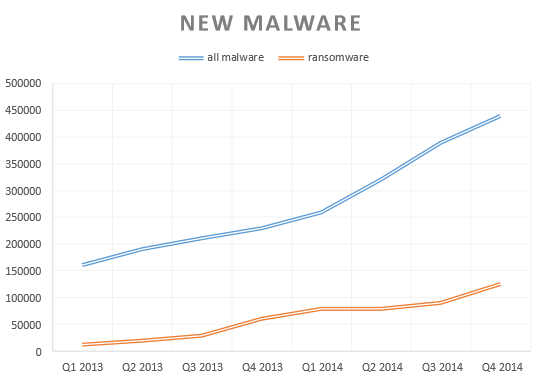
\includegraphics[width=0.45\textwidth]{increase}
\end{figure}

They found most prominently:
\begin{itemize}
\item There are two main Ransomware families (specific pieces of software which have developed over the years). Both with highlighted traits, these are:
\begin{enumerate}
\item TorrentLocker - A Ransomware exclusively distributed by email, and uses the infected user's email address list to distribute further.
\item CryptoWall - Communicates back to the attackers using the Tor network, to remain anonymous.
\end{enumerate}
\item There are a further 97 variants, most of which are related. Some are direct copies however.
\item 35.6\% of the attacks were made by Ransomware that do not perform encryption, but simply delete users files if they do not pay the ransom.
\item CyrptoWall infected 250,000 computers worldwide in the year of publishing (2015).
\end{itemize}Both of the described Ransomware families above are particularly sophisticated according to the author's findings, stating that they both use AES (Advanced Encryption Standard) to encrypt user data. This happens once a user is infected, and because of the high level of security AES was designed for (this method is used by the U.S. government to encrypt classified information for instance \cite{aes}), it makes any attempt at decrypting user data without paying extremely difficult. \par
Although other Ransomware use less sophisticated locking mechanisms such as standard Windows functions as described in the paper, a common user would still not be able to unencrypt the data without the help of good decryption software or with guidance from professionals. The paper noted that it in fact most Ransomware were not concentrating on the strength of the encryption, as long as it took away the ability for users to access files, then they could begin holding such users at ransom. In a whitepaper published by Boromium Security \cite{bromium}, file type targeting is something that can increase the efficiency and speed at which more vital files are encrypted. By only encrypting recently modified, new and common file-type files (as shown in Figure 2.), a Ransomware can cut its footprint and avoid anti-virus systems detecting major file system changes.
\begin{figure}[H]
  \caption{The number of file types encrypted by numerous Ransomware.}
  \centering
  \label{fig:files}
    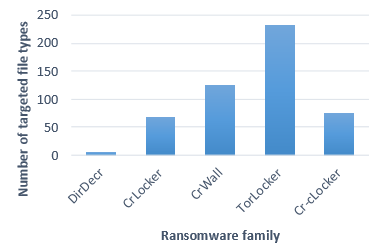
\includegraphics[width=0.45\textwidth]{files}
\end{figure}
The final aspect, and most important part to the process of an attackers infecting a user with the malware is the payment or ransom. In order to remain anonymous, and so that attackers cannot be traced, Bromium noted that nearly all Ransomware used BitCoins as payment. This secure and anonymous payment system allows anyone to send virtual cash through unique BitCoin addresses which can later be traded for cash. \par
Figure 3 shows the most common found way that Ransomware attacks happen. Though with nearly 40\% attacks now affecting multiple platforms, there is a constant shift in means of attacking.
\begin{figure}[H]
  \caption{An example flow of a Ransomware attack.}
  \centering
  \label{fig:order}
    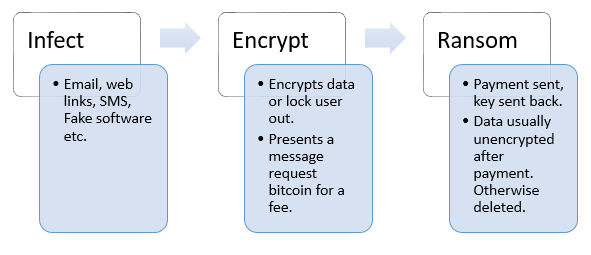
\includegraphics[width=0.45\textwidth]{order}
\end{figure}
\subsection{Transmission of malware}
Although the paper mentioned earlier (A look under the hood) goes into great detail of how Ransomware functions, and the statistics around them, the means at which users receive the malware is very brief in Kharraz's paper. In order to understand how Ransomware is transported, and how this relates to user responsibilities, other papers gave good insight. The Bromium whitepaper listed findings for most common Ransomware attacks:
\begin{itemize}
\item Spam or social engineering
\item Direct or indirect user download
\item Malware installation tools and botnets
\end{itemize}
Where these means of infection relate to the topic of this paper is in the fact that all three contain some user involvement. Without the user clicking on a suspicious link, downloading faulty software, or installing software with unwanted additional add-ons, it could be claimed that malware would not exists or exist in a different manner, as told by K. Wyk \cite{artical}. Because Ransomware realises heavily on user interaction, this is where this form of malware is required to look more professional than traditional viruses or spamming software. \par
The Bromium report highlights the professionalism that is shown from some of the Ransomware seen, and the increase is overall sophistication, making it more believable to be safe software of any kind. As mentioned in the abstract, emails produced to bring users to download the malware has been found to be increasing in sophistication too, with the use of correct user postcodes sent out. Because of this professionalism in the malware produced, software can almost seem to be on the side of the user when trapping them into a ransom. \par
\subsection{"al Ransomware victims}
Because the main objective of Ransomware attacks being money, attackers of this type of malware usually aim for high profile, wealthy victims. The Bromium report highlights this, saying that attacks will usually perform some research into potential victims, and accustom emails or phishing materials towards them specifically. \par
Although wealthier victims are attractive to attackers due to the better chance that they would be willing to pay ransoms, some reports suggest that a lot of attacks are performed on high profile individuals and organisations too. A report by ITProPortal \cite{pro-portal} argues that high profile organisations are becoming more attractive potential victims to attackers, and provides the example of a police department in Maine who were attacked and actually payed the ransom. It was reported that the attack invoked embarrassment of losing data, therefore forcing the organisation to pay. \par
By attacking large organisations, it goes back to the idea that with more money, they would be more willing to pay. It was found that 60\% of all Ransomware attacks were on companies. On the other hand, some Ransomware (such as cryptolocker) attacks individuals more often, and aims to spread further, requesting smaller amounts of ransom from users. By doing this more often than to larger, less cost sensitive victims, the attackers can still achieve great amounts from attacks. Although the success rate may go down by applying phishing emails to a wide group of users (though as mentioned, recent developments have allowed attackers to get basic user details like postcodes), the range of user skills can cover more, meaning basic users who would be more inclined to pay would be found by the Ransomware.

\subsection{The psychology of a Ransomware victim}
A quote made by James Scott from the Institute for Critical Infrastructure Technology said that "Ransomware is more about manipulating vulnerabilities in human psychology than the     adversary's technological sophistication". Although the user may be at ransom with their data, the way in which attackers attempt to convince users to pay is by gaining the trust of a user. To do this various insightful ways have been produced over recent years, such as CryptoWall's method of giving a user one free decryption key in order to make it believable that the attackers actually have the ability to unlock the user's files \cite{paper4}. \par
Images of various Ransomware shown in the Bromium report actually show clear and helpful instructions on how to make payment, and how to decrypt files, again instilling trust with the user. By providing trust, a user will me more inclined to pay, which sets this type of malware apart from any others. Having a user wanting to pay the attackers rather than the attackers having to attempt to steal financial data using more aggressive software makes the work of an attacker in this situation much easier, and more profitable if the attacker can reach the Ransomware to many users. \par

\section{Human errors}
Because humans build and use machines, a mistake by a machine can usually be related back to an error by the human who built it. Therefore, the weakest part of any system appears to be the users, as stated by A Sharaki (Human errors in computer related abuses) \cite{paper1}. The paper points out a number of ways a person can affect the usage and vulnerability of the system, which are not limited to:
\begin{itemize}
\item Fooled, distracted or persuaded
\item Blackmailed- heavily related to Ransomware
\item Be affected by human characteristics such as being tired, idle or apathetic
\end{itemize}
Any of the above can benefit viruses of any kind, making it easier for them to infiltrate computer and networks. Human errors are said to be distinguishable into two types, slips and lapses. Slips could be something such as attaching a wrong file in an email, whilst a lapse would be leaving systems open or unlocked. These two definitions were coined by James Reson (1990) \cite{james}, who compared mistakes to errors, stating that the mistake in the two cases mentioned previously was in not having an adequate plan for checking emails are from reliable sources. A mistake is therefore something that can heavily impact the possibilities of human error. By eradicating mistakes and being more prepared for human error, computer related abuses would be less frequent. \par
In addition to this, the paper by Sharaki noted that human error is part of a human behaviour and that because of many preceding events (or mistakes as mentioned), it may not be the fault of the human. \par
Designers and developers should be aware of the human errors issue, and therefore build mechanisms for dealing with possible errors according to Sharaki. Even if a developer was to create a perfect system with no bugs, or a system that did exactly what it was supposed to do, they should always be designed with any possible misuse in mind. For instance, without blocking every email that comes into a user's system, there will always be a finite number of suspicious emails that will come through the spam filter, and at that point the security lies with the user. In the case of Ransomware, because of the growing advancement of email authenticity this is one example of a hard to avoid mistake without further user training. \par
In addition to the developers, Sharaki also asks for ISPs (Internet Service Providers to protect against spyware and viruses by actively stopping suspicious network activity, which take yet more room for error out of the hands of users.) \par
As stated already, even with many precautions in place, unintentional threat still remains an increasing problem for many organisations or stand-alone users. Alphonso Price (Human factors in information security, 2015) \cite{human-factors} gathered some statistics on mistakes made by users resulting in issues for their respective organisations, and found that 57\% of employees believed that breaches in security caused by accidental or careless users are more damaging as breaches caused by intentionally malicious users. The author believed the reasoning for this lied with the fact that it is easier to predict the subject of attack when done purposely, but unintentional mistakes from other users are unpredictable and harder to foresee. \par
\subsection{Human errors as a factor in attacks}
By combining the proceeding examples of human errors in computing with how Ransomware attacks generally flow, some correlation can be seen. Several statistical reports on the web have begun to identify this, such as an article from the Visual media alliance \cite{visual-media} who have combined the increase in Ransomware attack numbers with the increase in users and amount of errors resulting. One concerning statistic given is that there is an 11\% chance of an employee clicking on a phishing link (Ransomware or other phishing software), and letting the program entry into the system or company wide database. \par
Another frightening statistic provided by the report highlights the amount of time taken for attacks to take place. With most emails (including phishing emails) opened within one minute, it makes controlling the human factor of attacks much more difficult, and gives less time to prevent code reaching a system. For Ransomware, this is especially concerning due to the quick nature of the malware. As shown in previously in this paper, Ransomware is becoming more and more adept at picking efficient ways of attacking a file system when encrypting, by targeting less, but more important files. Because phishing emails are opened so quickly, Ransomware is given an ideal amount of time to attack and lock out a user. \par
Because Ransomware leaves less of a trail on a system when encrypting or locking out a user, the security of an organisation or user may not be enough, and relying on them may not be enough. The paper identifies this, and it is down to user skill or knowledge to help reduce threat levels.
Reinforcing the idea of attacks being strongly correlated to human error, Verizon's director of global security services stated that "Despite advances in information security research, we continue to see many of the same errors we've known for more than a decade now".  This was said alongside the claim that 95\% of cybersecurity incidents were due to human error \cite{human-error}.  

\section{Legal and ethical consequences of Ransomware}
It is clear that the exposure of Ransomware is not only breaking laws, but is unethical. Although it is easy to see which laws are being broken from writing and releasing Ransomware software, there is also the implications for users or organisations that are allowing this malware to effect other users. This section looks at laws and ethical situations from the writing of Ransomware through to the exposure of it. \par
The Computer Misuse Act 1995 is designed to deal with hackers and viruses, and is one law that Ransomware breaks. Buy writing the malicious code designing to access computer material with intent to commit further offences (in this case, commit fraud) is one of the offences for which this law covers. In addition, it is generally thought of as extremely unethical by society to take advantage of a user's trust in order to receive payment from them. Because the software is essentially a scam, it is easy to pin several UK and international laws on any found attackers, but due to the anonymous protection (communicating through Tor, and payments through BitCoin) that attackers use, cases of Ransomware have very rarely resulted in charges. \par
On the other hand, organisations or internet services providers who do not provide sufficient protection against attacks may be breaking the Data Protection Act 1998. The act, which requires anyone holding another users' data, should make it as secure as possible. Although in some cases the law does not apply (such as individuals holding their own data), an ethical standpoint has been used in past Ransomware attacks where employees of attacked companies have accused their organisation of having too weak a security, and placing too much risk in the hands of themselves.

\section{Mitigation findings}
From the research performed into how a typical Ransomware attack takes place, and how human error appears to effect the circumstances of an attack, further study has been done into what means of prevention is applicable to this form of malware, both technically and individually. \par
There has been a rising number of papers looking at fighting Ransomware, and while most detail means of stopping Ransomware through the use of programs and other technology, most papers also include advice on how users should avoid getting infected in the first place. These papers suggest the need to prevent Ransomware by fixing the most error prone part of any system, the user habits. This section looks at both prevention mechanisms.

\subsection{Ransomware mitigation}
All papers in this topic suggest means of reducing the chance of Ransomware attacks, one such paper was a white paper by R. Lawhawn {paper3}, which looked directly at reducing the risk of attacks by various technological means.  The first of which is through the use of high quality antivirus software, one which offers file-based protection. Because Ransomware usually attacks files, detecting changes in a wide range of files could help detect a possible attack. \par
Alongside this, scanning emails and attachments before allowing a user to open them would catch a lot of Ransomware before it has the chance to start running. The best way of ensuring emails are scanned is to keep on top of any software updates and patches to the operating systems. By doing this, virus identifiers are up to date, and can help identifying the most popular Ransomware. \par
Although as mentioned in this report that newer Ransomware are using AES for their encryption, some are still using older simpler encryption methods that can now be broken by basic decryption software. The author highlights this as one of the first things to do after an attack, to attempt to retrieve data. \par
One method of mitigation can mean that before and after an attack, a user's data is still safe. Backups of a user's data can mean that if an attack did happen, the user would then be able to wipe a machine, and simply ignore the threat. The author does point out though that as simple as this is, there are still risks attached to it:
\begin{itemize}
\item Not backing up data regularly could mean data is still lost
\item Critical or sophisticated systems may not always be possible to be wiped and restarted
\item The Ransomware may take a copy of the user's data, and still hold them ransom
\end{itemize}
Amin Kharra also talks about API call monitoring \cite{paper4}, and looks at the use of the network when an attack is taking place. Kharra found in their research that a lot of Ransomware uses Windows API functions to lock desktop and make them unusable. But my monitoring a range of API calls, a classifier could be trained to detect suspicious sequence of calls. By training a classifier with samples gained from previous reports, a simple but effective program could learn when and how attacks were taking place, then informing he user at that time. \par
The author, alike Lawhawn, mentions the use of monitoring file system activity. Both file-deleting and file-encrypting Ransomware leave footprints when performing attacks, and therefore by monitoring the MFT (Master File Table), attacks can be easier detected. Although both papers mention this, the second goes into much more detail, giving explanations on how the MFT works, and how by monitoring MFT records that Ransomware can be prevented before harm is done. 

\subsection{Human error mitigation}
As mentioned throughout this paper, human errors are seen as being a large part of the process is Ransomware attacker's efforts. Therefore, there are a number of prevention strategies that look at the general concept of reducing these errors and mistakes. Lawhawn continues in his paper about reducing the risks of Ransomware, and goes onto the exact view of the users who allow the Ransomware to attack. The first of his recommendations are in the training of users. A well informed user is much less likely to be infected with Ransomware than one who is not. He notes that the most integral instinct knowledge that users should have is the capability to see when an email or link looks suspicious.\par
Users who are able to decide when an email may contain a virus, such as an attachment with a suspicious suffix (zip, exe etc.) will be at much less risk. Lawhawn also recommends that if an unknown file is received, the user could call or inquire through other means with the sender before opening. This way, any spoofing or hijacking of emails (as performed by CryptoLocker) can be mitigated. As for links and web addresses, and links in emails can be hovered over to find out the full address, while addresses are becoming easier to pre-scan with a range of web browsers today. \par
Kharra's paper has a more developer driven standpoint, which considers the protection developers of email clients, browsers and operating systems should offer users.  Where Lawhawn mentioned users checking emails before opening them, Kharra believes this more relies on the quality of email scanning. He also thinks that email clients should be more responsible for scanning errors, and filtering them accordingly. \par
Internet service providers are thought to also have the opportunity to reduce Ransomware attacks according to the paper by Kharra, saying that suspicious activity over the network should be tracked, and that phishing and transmission of viruses should be caught by the provider before it reaches the end user. \par
He does however believe in creating regular back-ups of systems, and leaves the responsibility with the users. A good user should have an automated back-up set up on their system, and any systems connected to the user's own machine should also be backed up, to ensure damage is not wide spread. As mentioned previously, although backups are the most inconvenient option, this is one key mitigation strategy that will hinder attacker's ability to force payment in return for decrypting or unlocking a user's machine.
Mentioned in the paper, an alternative approach to in house training and individual training could be to hire external sources to enhance the security of a user's machine. More and more companies choose to out-source their security needs, and there are examples of this across the Internet. One such security firm, who specialises in Ransomware protection claims to pay the attacker their ransom amount if they fail to protect the user \cite{ransom}.

\subsection{Mitigation drawbacks}
With all of the above described mitigation strategies, there are negatives to each. For instance, by taking more security out of the hands of the user and to email spam filters, there is the possibility of emails being incorrectly being marked, or lost. By forcing users to check each email by contacting the sender can be very time consuming also. This goes the same with backups, where a normal user may not have time or space to create a daily backup of their system, therefore middle ground must be found. \par
There is the debate of taking too much control from a user when it comes to security, such that Kharra believes that users may not know what the system is doing for them, in terms of scanning personal files or automatically checking links for them. With this, he thinks that relying on machines too much is dangerous, and could in fact weaken a typical user’s ability of seeing when one scenario looks suspicious or not. In the case of Ransomware, and in removing more control from a user, it might mean that a malicious email makes it through the system, only for the user to then assume it is none-malicious. Because of the sophistication of Ransomware, spam filters may not always work, therefore increasing the chance of this scenario. \par
In addition to these hindrances, the cost and effort required to keep up the protection against Ransomware attacks would increase. Regular back-ups, user training, and anti-virus software all adds to the cost to the end user.

\section{Conclusion}
Following discussions of how both human errors contribute to the effect of viruses, malware and other attacks on machines, there is good evidence in a range of papers that human error has been contributing towards the rise in Ransomware. As shown in earlier parts of this paper, the increase in the amount of users has given attackers a wider spread of user abilities, therefore allowing them to subject less adept users with the malware. As more users are open to more and more forms of communication, the ways in which users are able to receive Ransomware has also increased. \par
Looking at the future of Ransomware, it appears that the trend displayed at the beginning of this report will continue, and C. Talos \cite{talos} gave his insight into the possible advancements in Ransomware. They were:
\begin{itemize}
\item Custom selective directories and files could be encrypted on command- This would mean Ransomware would be even more efficient at targeting important files.
\item More advanced contact means to the attackers- This would further drive users to pay the ransom, and with increased contact and support, more trust would be built up with the attackers.
\item Rate limiting- This would mean attackers could limit the rate at which file are encrypted, meaning the malware would be much harder to detect.
The writer here highlights the gain of trust between attackers and victims, mentioning that exploiting users more in future is a key area where attackers will concentrate. 
\end{itemize}

\ifCLASSOPTIONcaptionsoff
  \newpage
\fi

\begin{thebibliography}{1}

\bibitem{bbc-Ransomware}
BBC Technology News, \emph{The Ransomware that knows where you live}, \hskip 1em plus
  0.5em minus 0.4em\relax \url{http://www.bbc.co.uk/news/technology-35996408} BBC. 2016.
  
\bibitem{paper4}
A.~Kharraz et.al, \emph{Cutting the Gordian Knot: A Look Under the Hood of Ransomware Attacks
},\hskip 1em plus
  0.5em minus 0.4em\relax Northeastern University, Boston, USA. 2015.
  
\bibitem{aes}
Tech Target, \emph{Advanced Encryption Standard (AES)}, \hskip 1em plus
  0.5em minus 0.4em\relax \url{http://searchsecurity.techtarget.com/definition/Advanced-Encryption-Standard}. 2014.
  
\bibitem{bromium}
V.~Kotov and M.~ Rajpal, \emph{Understanding  Crypto-Ransomware},\hskip 1em plus
  0.5em minus 0.4em\relax Bromium Inc, 2015.
  
\bibitem{artical}
K.~van Wyk, \emph{Blaming Users for Virus Chaos?}, 3rd~ed.\hskip 1em plus
  0.5em minus 0.4em\relax \url{http://www.esecurityplanet.com/views/article.php/3377201/Blaming-Users-for-Virus-Chaos.htm}, 2004.
  
\bibitem{pro-portal}
D.~Balaban, \emph{High profile ransomware victims: No one is safe – You could be next},\hskip 1em plus
  0.5em minus 0.4em\relax \url{http://www.esecurityplanet.com/views/article.php/3377201/Blaming-Users-for-Virus-Chaos.htm}, 2016.
  
\bibitem{paper1}
A.~Sharaki and M.~Nikaram , \emph{Human Errors in Computer Related Abuses},\hskip 1em plus
  0.5em minus 0.4em\relax Journal of Theoretical and Applied Information Technology Vol 47 No 1. 2013.
  
\bibitem{james}
J.~Reason, \emph{Human Error},\hskip 1em plus
  0.5em minus 0.4em\relax Cambridge University Press. 1990.
  
\bibitem{human-factors}
A.~Price and Y.~Choi, \emph{Human Factors in Information Security},\hskip 1em plus
  0.5em minus 0.4em\relax International Journal of Computer and Information Technology, Vol 04 Issue 05. 2015.

\bibitem{visual-media}
Visual Media Alliance, \emph{Cyber Threat Mounts with Human Error and Ransomware}, \hskip 1em plus
  0.5em minus 0.4em\relax \url{http://main.vma.bz/insurance/cyber-threat-mounts-with-human-error-and-ransomware}, 2013.
  
\bibitem{human-error}
E.~Mitchell, \emph{Combatting human error in cybersecurity}, \hskip 1em plus
  0.5em minus 0.4em\relax \url{https://www.helpnetsecurity.com/2015/08/24/combatting-human-error-in-cybersecurity/}, 2015.
  
\bibitem{paper3}
R.~Lawhorn, \emph{Ransomware: How to Reduce Risk and Protect Your Business },\hskip 1em plus
  0.5em minus 0.4em\relax Clare Computer solutions. 2016.
  
\bibitem{ransom}
KnowBe4, \emph{We Will Pay Your Crypto-Ransom If You Get Hit With Ransomware},\hskip 1em plus
  0.5em minus 0.4em\relax \url{https://www.knowbe4.com/ransomware-cryptolocker-guarantee}. 2016.
  
\bibitem{talos}
C.~Talos, \emph{Ransomware: Past, present and future},\hskip 1em plus
  0.5em minus 0.4em\relax \url{http://blog.talosintel.com/2016/04/ransomware.html#ch5}. 2016.
  
\end{thebibliography}

\end{document}


